\documentclass{article}
\usepackage{amsmath}
\usepackage{tikz}
\usetikzlibrary{calc}

\begin{document}

\begin{figure}[h]
    \centering
    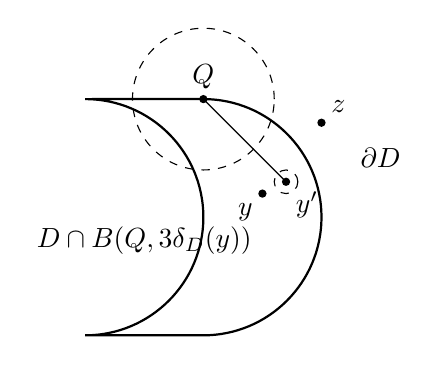
\begin{tikzpicture}[scale=1.5]
        % Define points
        \coordinate (Q) at (0, 1);
        \coordinate (z) at (1, 0.8);
        \coordinate (y) at (0.5, 0.2);
        \coordinate (y') at (0.7, 0.3);
        
        % Draw the boundary of D
        \draw[thick] (Q) arc (90:-90:1) -- (-1,-1) arc (-90:90:1) -- cycle;
        \node at (1.5, 0.5) {$\partial D$};
        
        % Draw the intersection with the ball B(Q, 3\delta_D(y))
        \draw[dashed] (Q) circle (0.6);
        \node at (-0.5, -0.2) {$D \cap B(Q, 3\delta_D(y))$};
        
        % Draw the smaller ball around y'
        \draw[dashed] (y') circle (0.1);
        
        % Draw the point z
        \fill (z) circle (1pt);
        \node at (z) [above right] {$z$};
        
        % Draw the points y and y'
        \fill (y) circle (1pt);
        \fill (y') circle (1pt);
        \node at (y) [below left] {$y$};
        \node at (y') [below right] {$y'$};
        
        % Draw the line segment QQ'
        \draw (Q) -- (y');
        
        % Label Q
        \fill (Q) circle (1pt);
        \node at (Q) [above] {$Q$};
    \end{tikzpicture}
    \caption{Illustration for Lemma~\ref{lem:gdint}. The boundary Harnack principle cannot be used to estimate increments between $y$ and $y'$ because of the singularity at $z$. Instead we show regularity in the smaller ball using harmonicity in the larger ball.}
    \label{fig:gdint}
\end{figure}

\end{document}